\documentclass{beamer}

\usepackage[utf8]{inputenc}
\usepackage{default}
\usepackage{amsmath}

\title{A Tutorial on Multigrid Methods}
\author{Philip Greggory Lee}
\institute{
 Electrical Engineering and Computer Science\\
 Northwestern University\\
 Evanston, IL 60208
}

\AtBeginSection
{
 \begin{frame}{Outline}
  \tableofcontents[currentsection]
 \end{frame}
 \addtocounter{framenumber}{-1}
}

\providecommand{\defeq}{\stackrel{\Delta}{=}}
\providecommand{\abs}[1]{\Bigl\lvert #1 \Bigr\rvert}
\providecommand{\norm}[1]{\left\lVert #1 \right\rVert}

\begin{document}

\begin{frame}
 \titlepage
\end{frame}

\begin{frame}{Outline}
 \tableofcontents
\end{frame}
\addtocounter{framenumber}{-1}

\section{Introduction}%========================================================

\begin{frame}{The Problem}
 \begin{itemize}
  \item Suppose we have a linear system whose variable $u$ represents a discretization
        of a function $g(x)$ on a regular grid.
  \begin{align}
   Au=f
  \end{align}
  \item As the level of discretization grows, so does the size of the system.
  \item In many typical cases, the condition number of $A$ grows with the
        square of the size of $u$.
  \item Simple linear solvers therefore slow down dramatically as the resolution
        increases.
 \end{itemize}
\end{frame}

\begin{frame}{The Intuition}
 \begin{itemize}
  \item Why should this be the case?
  \item In most cases, increasing the resolution does not \textit{really}
        introduce more complexity into the problem.
  \item Is there any way we can take advantage of the notion of
        \textit{resolution} of the solution $u$ in a principled way?
  \item The answer is yes, and we will explore a class of ways to do so called
        \textbf{multigrid methods}.
 \end{itemize}
\end{frame}

\begin{frame}[allowpagebreaks]{Notation}
 
\end{frame}

\section{The Motivating Example}%==============================================

\begin{frame}[allowframebreaks]{1D Laplace Problem}
 \begin{itemize}
  \item A simple example that serves to illustrate the major points of this
        tutorial is the Laplace equation in 1D with Dirichlet boundary
        conditions.
  \begin{align}
   Au &= f, \; \text{where} \label{eq:laplace} \\
   Au &= -\Delta u = - \nabla \cdot \nabla u, \; \text{and} \nonumber \\
   f &= 0 \nonumber \\
   \text{s.t.} \; & u_0 = u_{n+1} = 0 \nonumber
  \end{align}
  \item In this case, the Laplace operator $\Delta$ can be represented by
        convolution with the kernel $[1,-2,1] = [1,-1]\ast[1,-1]$.
  \begin{figure}
   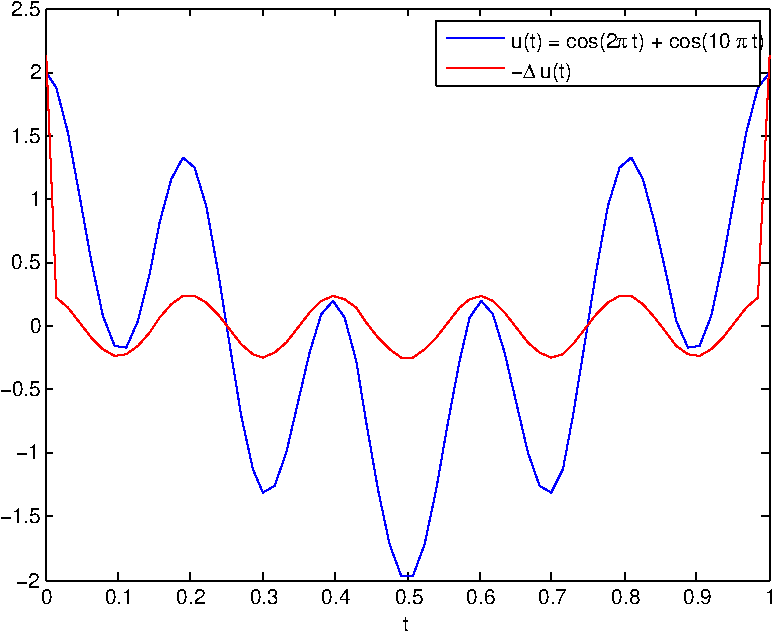
\includegraphics[width=6cm]{images/laplaceOperatorExample.pdf}
  \end{figure}
  \item Strictly speaking, if we are approximating the continuous Laplace
        operator, then the kernel is $\frac{1}{h^2}[1,-2,1]$ if the samples
        are spaced $h$ units apart. It's just a scaling factor.
  \item For simplicity, we will assume that the discrete variables are spaced
        $h = 1/(n+1)$ units apart so that $u$ represents a function over the
        unit interval $[0,1]$.
  \item Equation $i$ of \eqref{eq:laplace} reads:
  \begin{align}
   -u_{i-1}+2u_i-u_{i+1} = 0, \; \forall 1 \leq i \leq n
  \end{align}
  \item Notice that the boundary conditions $u_0 = u_{n+1} = 0$ are incorporated
        into this system.
  \item In this particular case, the eigenfunctions of A are $v^h_{(k)i} = \sin(k \pi ih)/h$,
        with $1 \leq i,k \leq n$ and its eigenvalues range from $\lambda_1^h \approx \pi^2 h^2$ to
        $\lambda_n^h \approx 4-h^2$.
  \item Notice that the condition number
        $\kappa(A) = \lambda_n^h / \lambda_1^h \approx 4/(\pi^2h^2) = 4(n+1)^2/\pi^2$.
  \item So, the condition number grows as $O(n^2)$ with system size $n$.
  \item We will see that this is the major problem facing standard linear solvers.
  \begin{figure}
   \begin{tabular}{cc}
    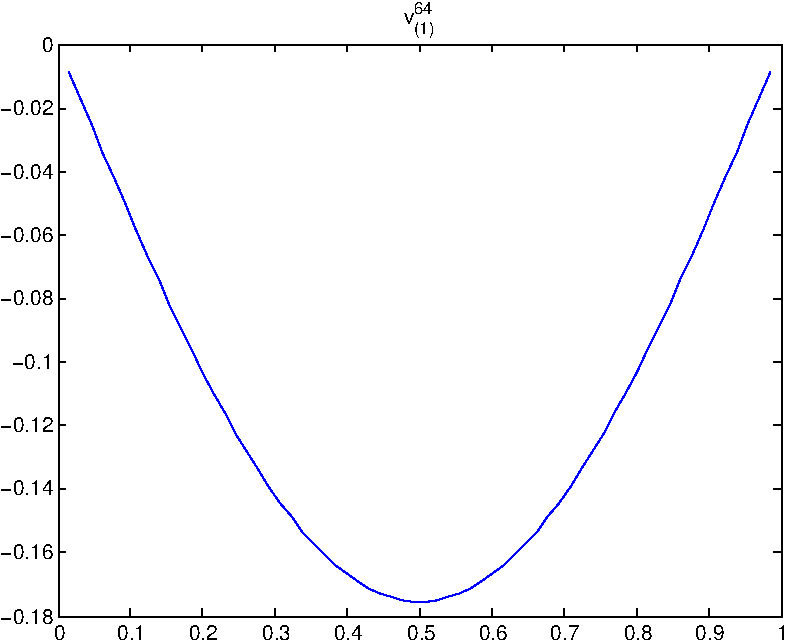
\includegraphics[width=4cm]{images/v64_1.pdf} & 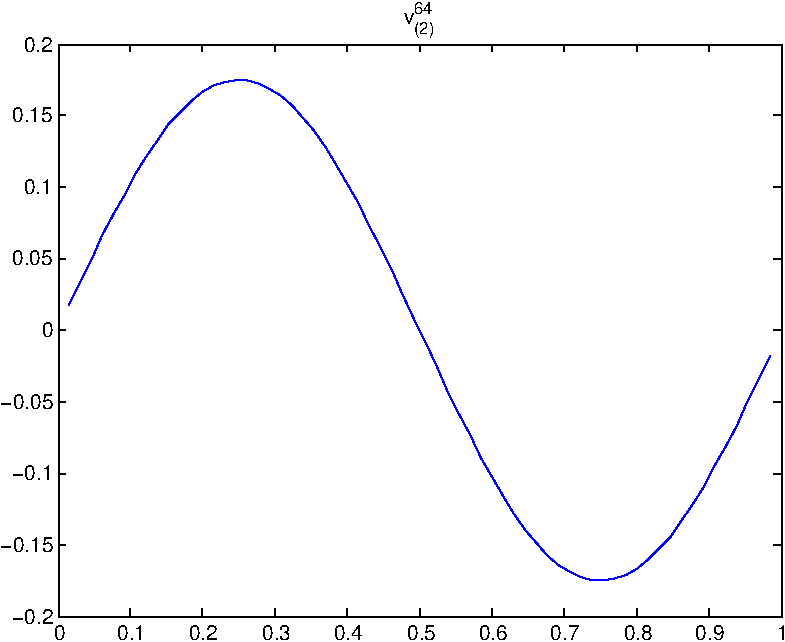
\includegraphics[width=4cm]{images/v64_2.pdf} \\
    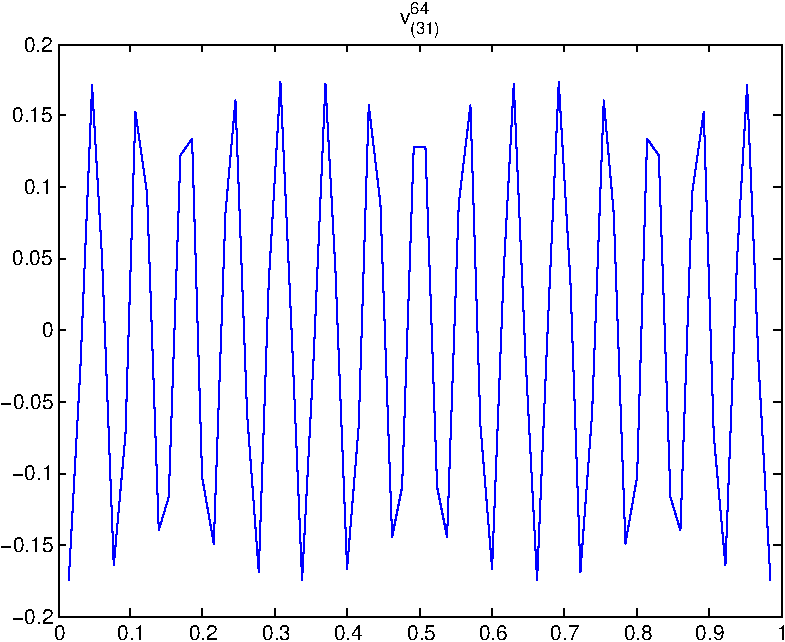
\includegraphics[width=4cm]{images/v64_31.pdf} & 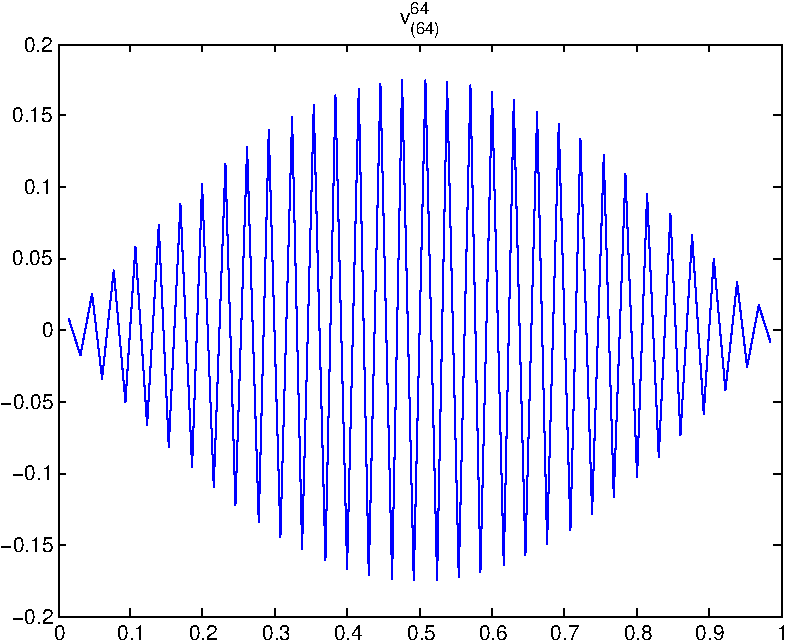
\includegraphics[width=4cm]{images/v64_64.pdf}
   \end{tabular}
   \caption{Eigenfunctions of $A$ when $n=64$ ($h=1/65$).}
  \end{figure}
 \end{itemize}
\end{frame}

\section{Relaxation (Iterative Methods)}%======================================

\begin{frame}{Jacobi Method}
 \begin{itemize}
  \item How can we solve such a problem?
  \item A first stab is just to satisfy each equation independently:
  \begin{align}
   u_{i(\text{new})} \leftarrow \frac{u_{i-1}+u_{i+1}+f_i}{2}
  \end{align}
  \item \textbf{Remember}: for us, $f_i=0$.
  \item This is the strategy of the \textbf{Jacobi Method}.
  \item Formally, if $D$, $-L$, and $-U$ are the diagonal, lower, and upper
        triangular parts of $A$ resp., then $A=D-L-U$ and the Jacobi Method is:
  \begin{align}
   u \leftarrow D^{-1}(L+U)u+D^{-1}f
  \end{align}
 \end{itemize}
\end{frame}

\begin{frame}[allowframebreaks]{Relaxation}
 \begin{itemize}
  \item In general, we call any method of the following form \textbf{relaxation}:
  \begin{align}
   u \leftarrow G(u) = Ru+g.
  \end{align}
  \item If $\hat{u}$ is the solution, it must be the case that it is a fixed
        point of the iteration: $\hat{u} = R\hat{u}+g$.
  \item For analysis, it is useful to make the transformation
  \begin{align}
   e &\defeq \hat{u}-u \\
   r &\defeq f-Au
  \end{align}
  \item This means the original problem is transformed to $Ae=r$.
  \item Note that $\hat{e} = 0$.
  \begin{align}
   e_{\text{new}} &= \hat{u} - (Ru+g) \\
                  &= \hat{u} - R(\hat{u}-e) - g \\
                  &= \hat{u} - (\hat{u}-g) + Re - g \\
                  &= Re
  \end{align}
  \item So, the error evolution is given by $e \leftarrow Re$.
  \item Since this iteration must converge to 0, a sufficient condition for
        convergence is $\rho(R) < 1$, where $\rho$ is the spectral radius.
  \item So, for any consistent norm $\norm{\cdot}$, a simple upper bound on the convergence rate is
  \begin{align}
   \frac{\norm{e_{\text{new}}}}{\norm{e}} \leq \rho(R)
  \end{align}
 \end{itemize}
\end{frame}

\begin{frame}[allowframebreaks]{Jacobi Convergence Rate}
 \begin{itemize}
  \item Note that for the Jacobi method, the iteration matrix $R=D^{-1}(L+U)$.
  \item What is $\rho(R)$?
  \item We will prove that $\rho(R) \leq 1-\frac{\pi^2 h^2}{2}$
  \pagebreak
  \begin{theorem}
   $\rho(R) \leq 1-\frac{\pi^2 h^2}{2}$
   
   \begin{proof}
    Proof by contradiction. Suppose $\exists y$ s.t. $Ry = (1-\frac{\pi^2 h^2}{2}+\epsilon)y$.
    Then,
    \begin{align}
     Ay &= (D-DR)y = Dy-DRy \nonumber \\
        &= 2y - 2(1-\frac{\pi^2 h^2}{2}+\epsilon)y \nonumber \\
        &= (\pi^2 h^2 - 2 \epsilon) y
    \end{align}
    So, $y$ is an eigenfunction of $A$ with eigenvalue $\pi^2 h^2 - 2 \epsilon$.
    But this is a contradiction since $\lambda^h_1 = \pi^2 h^2$.
   \end{proof}
  \end{theorem}
  \pagebreak
  \item So, using the Jacobi method, the convergence rate slows quadratically
        with $n$.
  \begin{figure}
   \begin{tabular}{cc}
    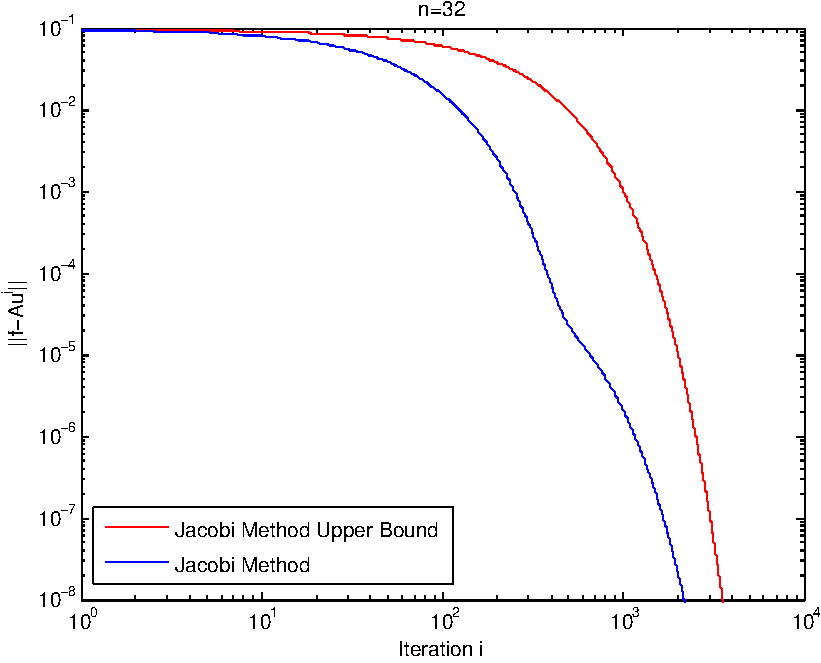
\includegraphics[width=4.5cm]{images/jacobiConvergence_32.pdf} & 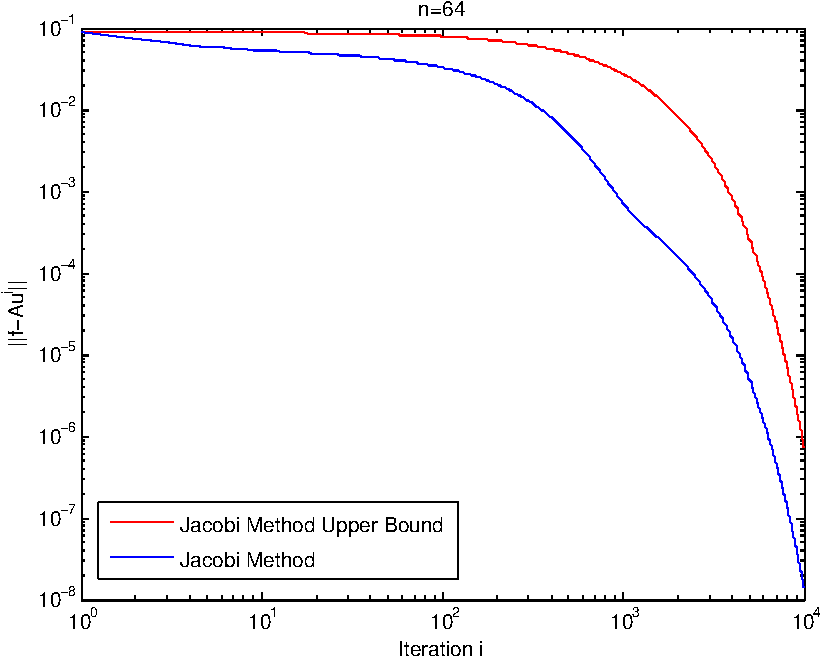
\includegraphics[width=4.5cm]{images/jacobiConvergence_64.pdf}
   \end{tabular}
   \caption{Convergence rate and upper bound for convergence rate of Jacobi
            method on our model problem.}
  \end{figure}
  \item In fact, the eigenvalues of $R$ range from $\mu_1^h \approx 1-\pi^2h^2/2$
        to $\mu_n^h \approx -\mu_1^h$.
  \item \textbf{Important}: notice that low-frequency eigenfunctions ($i\ll n$)
        of $A$ correspond to $\mu_i \approx 1$ and high-frequency eigenfunctions
        ($i \approx n$) correspond to $\mu_i \approx -1$.
  \item This means that very high and very low frequency components of error $e$
        are very slow to converge.
  \item On the flip side, mid-frequency components correspond to
        $\mu_i \approx 0$ and converge very quickly indeed.
  \begin{figure}
   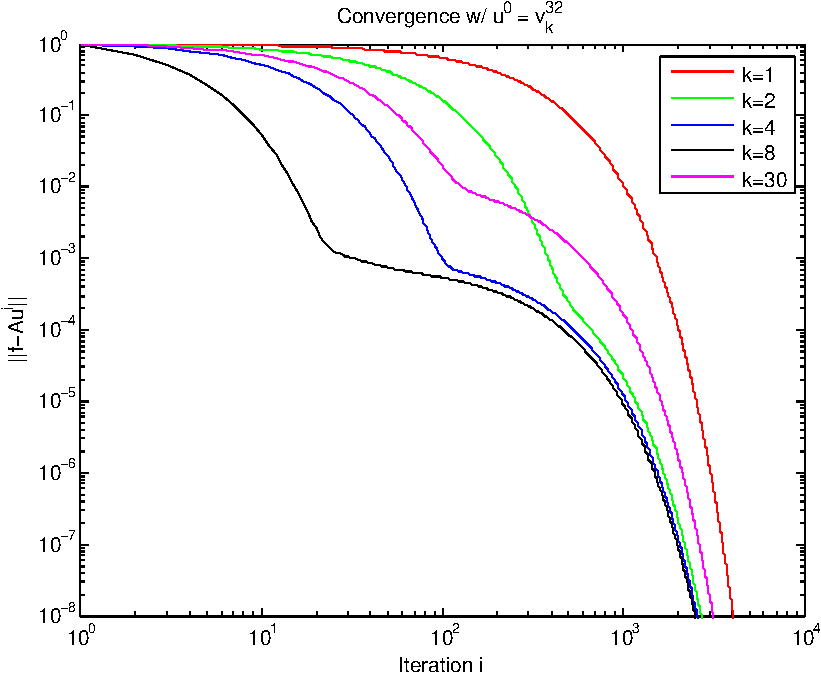
\includegraphics[width=6cm]{images/jacobiConvergence_freq.pdf}
   \caption{$n=32$. High and low-frequency components ($k \approx 1$ or
            $k \approx 32$) converge slowly, while mid-frequency components
            converge quickly.}
  \end{figure}
 \end{itemize}
\end{frame}

\begin{frame}[allowframebreaks]{Gauss-Seidel}
 \begin{itemize}
  \item Another simple relaxation method is \textbf{Gauss-Seidel}.
  \item Instead of always using the old values of $u$ to get $u_(\text{new})$,
        it uses the new values immediately after computing them to solve each
        equation.
  \begin{align}
   u_{i\text{(new)}} \leftarrow \frac{u_{i-1\text{(new)}}+u_{i+1}+f_i}{2}
  \end{align}
  \item In operator notation, this is
  \begin{align}
   u \leftarrow (D-L)^{-1}Uu + (D-L)^{-1}f
  \end{align}
  \item So, the iteration matrix in this case is $R=(D-L)^{-1}U$.
 \end{itemize}
\end{frame}

\begin{frame}[allowframebreaks]{Damped Jacobi}
 
\end{frame}

\section{Nested Iteration}%====================================================

\section{Basic Multigrid Methods}%=============================================

\section{Analysis}%============================================================

\section{Recent Work}%=========================================================

% References ==================================================================
\begin{frame}[allowframebreaks]
 \frametitle{References}
 \bibliographystyle{amsalpha}
 \bibliography{multigridrefs.bib}
\end{frame}

\end{document}
